\chapter{Conclusão}
\label{cha:conclusao}
\index{Conclusão}


Este estudo \textbf{investiga}, em caráter exploratório, as técnicas de 
reamostragem \textit{bootstrap}, \textit{bagging} e \textit{subagging}, 
aplicadas à Regressão Linear Múltipla (RLM) no contexto de calibração 
multivariada de amostras de aço-ligas, e \textbf{atende} integralmente 
aos objetivos propostos. % ALTERADO: adicionado "em caráter exploratório"
O trabalho \textbf{implementa} as abordagens 
utilizando a RLM como modelo base.

Os experimentos são conduzidos sob 
um protocolo metodologicamente controlado --- incluindo a otimização de 
parâmetros por validação cruzada 5-\textit{fold} aplicada exclusivamente 
ao conjunto de calibração ---, o que \textbf{garante} comparações justas 
e reprodutíveis entre os algoritmos \textit{RLM clássica}, 
\textit{RLM-bagging} e \textit{RLM-subagging}. Além do RMSEP, o estudo 
\textbf{incorpora} as métricas \gls{MAE} e R$^2$ à análise, ampliando 
a caracterização do desempenho preditivo de cada técnica.

%----------------------------------------------------------------------------

A análise comparativa entre os algoritmos \textbf{revela} variações de 
desempenho dependentes do analito avaliado e \textbf{confirma}, para 
este conjunto de dados específico, a inexistência de uma técnica 
universalmente superior. Para o Manganês 
(Mn), o RLM-\textit{subagging} ($k^* = 80\%$, $m^* = 10$) 
\textbf{apresenta} o menor RMSEP (0,0966), representando uma redução 
de 8,1\% em relação à RLM clássica. Para o Ferro (Fe), o 
RLM-\textit{bagging} ($m^* = 30$) \textbf{obtém} o melhor desempenho 
(RMSEP = 2,6406), com melhoria de 4,0\% sobre a RLM clássica.

Para o 
Níquel (Ni), o RLM-\textit{subagging} ($k^* = 60\%$, $m^* = 10$) 
\textbf{exibe} resultado marginalmente superior (RMSEP = 1,6003), com 
diferença de 0,25\% em relação à RLM clássica --- resultado que, dada 
a magnitude da diferença, deve ser interpretado com cautela no contexto 
do tamanho amostral disponível. % ALTERADO: adicionada ressalva sobre o Ni

Em contrapartida, para 
o Molibdênio (Mo) e o Cromo (Cr), a RLM clássica \textbf{demonstra} 
desempenho superior (RMSEP de 0,2633 e 1,0798, respectivamente), 
indicando que a complexidade adicional das estratégias de 
\textit{ensemble} não \textbf{resulta} em melhorias de precisão para 
esses analitos neste contexto.

%---------------------------------------------------------------------

A avaliação por meio do RMSEP, complementada pelo \gls{MAE} e pelo 
R$^2$, \textbf{possibilita} uma caracterização abrangente do desempenho 
preditivo. Todos os modelos \textbf{apresentam} coeficiente de 
determinação superior a 0,98 para todos os elementos, o que 
\textbf{evidencia} elevada capacidade preditiva para o conjunto de dados 
analisado. % ALTERADO: adicionado "para o conjunto de dados analisado"

Para Mn e Ni, o 
RLM-\textit{subagging} \textbf{exibe} dominância de Pareto sobre o 
RLM-\textit{bagging} --- por ser simultaneamente superior em acurácia 
(RMSEP e \gls{MAE}) e mais eficiente computacionalmente ---, o que 
\textbf{reforça} sua indicação preferencial em ambos os contextos. 
Para Mo e Cr, os resultados \textbf{sustentam} a adoção da RLM 
clássica, em razão de sua simplicidade e elevada eficiência 
computacional.

%--------------------------------------------------------------------

A análise da eficiência computacional \textbf{evidencia} diferenças 
significativas entre os métodos. A RLM clássica \textbf{detém} o melhor 
desempenho em termos de tempo de execução e \textbf{configura-se} como 
a abordagem mais eficiente. O RLM-\textit{subagging} \textbf{ocupa} 
posição intermediária e, em média, \textbf{supera} a velocidade do 
RLM-\textit{bagging} em 3,0 vezes (redução de 66,7\% no tempo), embora 
com variação entre elementos.

Em relação à RLM clássica, o 
RLM-\textit{subagging} \textbf{apresenta} custo até 19,5 vezes 
superior, enquanto o RLM-\textit{bagging} \textbf{mostra-se}, em média, 
22,1 vezes mais lento. O Cromo (Cr) \textbf{constitui} o único caso em 
que o RLM-\textit{subagging} não \textbf{apresenta} vantagem temporal 
sobre o RLM-\textit{bagging}, comportamento que o maior número de 
replicações ($m^* = 30$) \textbf{explica}.

%-------------------------------------------------------------------------

A investigação \textbf{indica} que o RLM-\textit{subagging} 
\textbf{configura-se} como a alternativa mais equilibrada entre precisão 
e eficiência para os dados analisados, sendo recomendado para Mn e Ni. 
% ALTERADO: adicionado "para os dados analisados"
Para Mo e Cr, os 
resultados \textbf{sustentam} a adoção da RLM clássica. O 
RLM-\textit{bagging} \textbf{mostra-se} preferível para Fe, embora o 
RLM-\textit{subagging} \textbf{atinja} desempenho preditivo equivalente 
em menos da metade do tempo. A relação de compromisso entre acurácia e 
tempo \textbf{atua} como elemento decisivo na seleção da técnica.

Do ponto de vista da engenharia de software, o trabalho também \textbf{atinge} seus
objetivos específicos: a arquitetura modular em três camadas independentes
(\texttt{models.py}, \texttt{components.py} e \texttt{app.py}) \textbf{satisfaz} o
requisito de modularidade (RNF01), enquanto a suíte de 92 testes automatizados
\textbf{confirma} a fidelidade comportamental entre o sistema Python reescrito e o
sistema Java legado (RNF03), consolidando a estratégia de migração incremental como
contribuição metodológica válida independentemente do domínio de aplicação.

Embora \textbf{alcance} resultados promissores, este estudo 
\textbf{apresenta} limitações pertinentes. O conjunto de dados 
\textbf{corresponde} a uma composição específica de aço-liga, analisada 
sob condições instrumentais particulares, o que \textbf{restringe} a 
extrapolação dos achados para outras composições, regimes amostrais ou 
configurações espectrométricas distintas. % ALTERADO: expandida a descrição das limitações

A razão de aproximadamente 42 preditores por observação no conjunto de 
calibração \textbf{caracteriza} um regime de alta dimensionalidade que, 
embora tratável pela pseudo-inversa de Moore-Penrose, \textbf{amplifica} 
a sensibilidade dos resultados à composição específica das amostras 
disponíveis. % ALTERADO: adicionada sentença quantificando o problema da dimensionalidade
Ademais, a análise \textbf{adota} exclusivamente a RLM 
como modelo base, e a dimensão reduzida do conjunto de calibração 
\textbf{impõe} restrições à generalização dos parâmetros identificados.

Como direcionamento para investigações futuras, este estudo 
\textbf{recomenda} a expansão do escopo para conjuntos amostrais maiores 
e diferentes classes de materiais, bem como a comparação com modelos 
preditivos alternativos, como \gls{PLS}, \gls{LASSO} e redes neurais, 
que \textbf{permitirão} avaliar se os padrões de desempenho aqui 
observados se sustentam em regimes mais generalizáveis. % ALTERADO: reescrita para conectar trabalhos futuros às limitações identificadas
A investigação \textbf{sugere}, ainda, a avaliação de 
técnicas de \textit{ensemble} mais sofisticadas, como \textit{boosting} 
e \textit{stacking}.

%\begin{figure}[htbp]
%	\centering
%		\includegraphics[width=1.000\textwidth]{G:/TecnicasDeReamostragem/Projeto_Integrador_III_Final/outros/fig/resultado_final.png}
%	\caption{Resultado final.}
%	\label{fig:resultado_final}
%\end{figure}

%--------------------------------------
%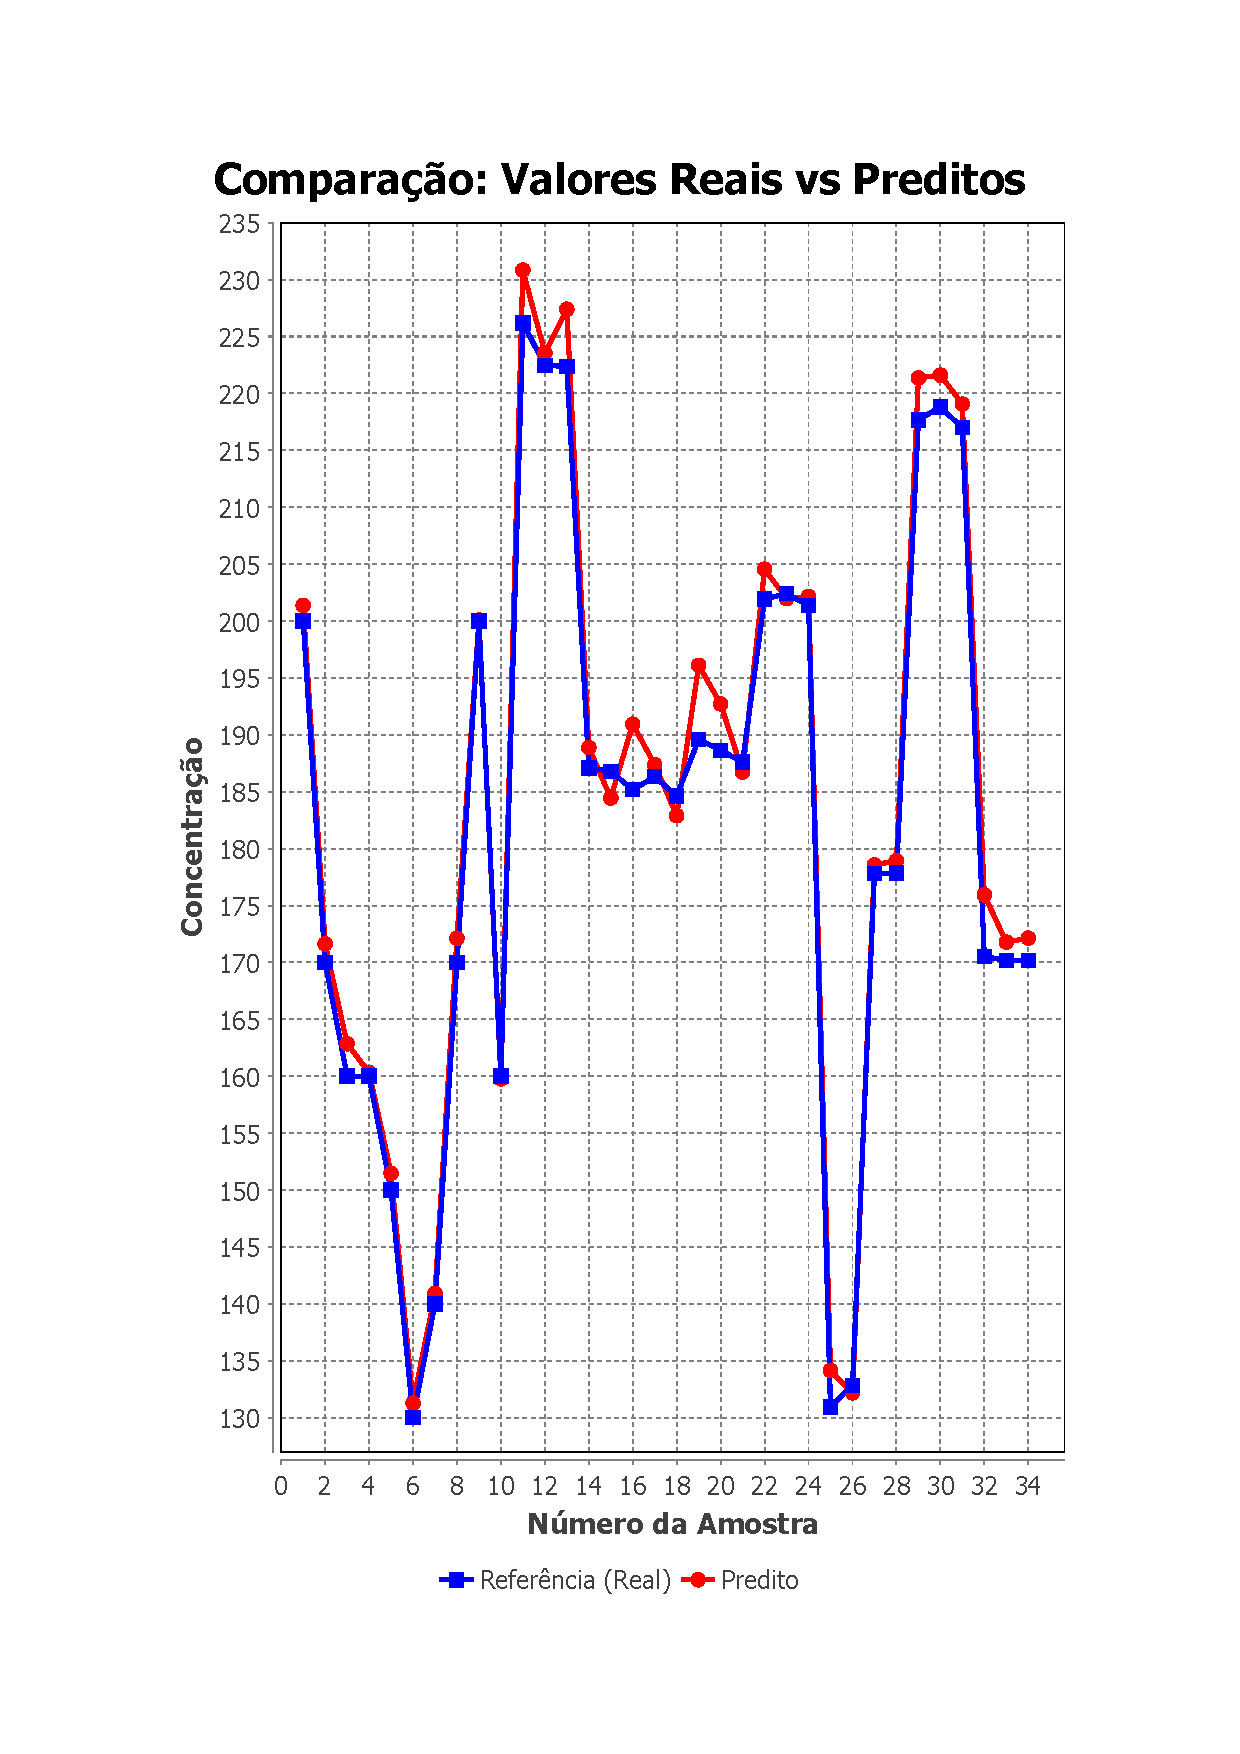
\includepdf[pages=-, scale=0.5]{./outros/fig/BootStrapRMSEPFe.pdf}  % Inclui todas as páginas
%--------------------------------------